\documentclass[11pt]{article}
\usepackage[margin=1in]{geometry}
\usepackage{amsmath,bm}
\usepackage{graphicx}
\usepackage{booktabs}
\usepackage{longtable}
\usepackage{url}
\usepackage{xcolor}
\usepackage[version=3]{mhchem}
\usepackage{authblk}
\usepackage{hyperref}

\renewcommand{\thepage}{S\arabic{page}}
\renewcommand{\thetable}{S\arabic{table}}
\renewcommand{\thefigure}{S\arabic{figure}}

\title{Supporting Information\\
DiffDock-Glide: a hybrid physics-based and data-driven approach to molecular docking}

\author[1,2]{Lukas Herron}
\author[3]{Jumana Dakka*}
\author[3]{Steven V. Jerome*}
\author[4]{Kun Yao}
\author[5]{Da Shi}

\affil[1]{Biophysics Program and Institute for Physical Science and Technology, University of Maryland, College Park, Maryland 20742, United States}
\affil[2]{Institute for Health Computing, University of Maryland, Bethesda, Maryland 20852, United States}
\affil[3]{Schr\"odinger Inc, 1540 Broadway Floor 24, New York, NY 10036, United States}
\affil[4]{Schr\"odinger Inc, 1 Main St, 11th Floor, Cambridge, MA 02142, United States}
\affil[5]{Schr\"odinger Inc, 9868 Scranton Rd Suite 3200, San Diego, CA 92121, United States}

\date{*E-mail: jumana.dakka@schrodinger.com; steven.jerome@schrodinger.com}

\begin{document}

\setcounter{secnumdepth}{0}

\maketitle

\section{Sensitivity Analysis of the Binding Site Conditioning Parameter $\gamma$}
\label{sec:gamma_sensitivity}

To empirically characterize the effect of the binding site conditioning parameter $\gamma$ on pose sampling distributions, we performed a sensitivity analysis across a range of $\gamma$ values using structures from the Posebusters benchmark set.\cite{buttenschoen2024posebusters} Five protein-ligand complexes were selected from the Posebusters benchmark (PDB IDs: 7KFO, 7M41, 7AKL, 7XEK, 7NF3). For each target, binding site parameters ($r_0$, $r_\mathrm{min}$, $r_\mathrm{max}$) were computed as described in the main text, using residues within 5~\AA\ of the crystallized ligand.

Poses were generated using DiffDock with $\gamma \in \{0.0, 0.1, 0.5, 1.0, 2.0, 5.0\}$. For each target-$\gamma$ combination, 40 poses were sampled, yielding a total of 1,200 poses across all conditions. The distance, $d$, from each sampled ligand centroid (center of geometry of heavy atoms) to the binding site center ($r_0$) was computed and normalized by $r_\mathrm{min}$ to enable comparison across targets with different binding site sizes.

Figure~\ref{fig:gamma_cdf} presents cumulative distribution functions (CDFs) of these normalized distances for each $\gamma$ value. The binding site boundary ($d/r_\mathrm{min} = 1$) is indicated by a vertical dashed line, and the legend reports the percentage of poses within this boundary for each condition. Without conditioning ($\gamma = 0$), only 47.9\% of poses fall within the binding site, with the remainder distributed broadly across the protein surface. Even modest conditioning ($\gamma = 0.1$) increases binding site occupancy to 60.4\%. At $\gamma = 0.5$ and the default value $\gamma = 1.0$, occupancy reaches 82.1\% and 82.8\%, respectively. Higher values ($\gamma = 2.0$, $\gamma = 5.0$) further increase occupancy to 89.5\% and 92.4\%.

\begin{figure}[h]
\centering
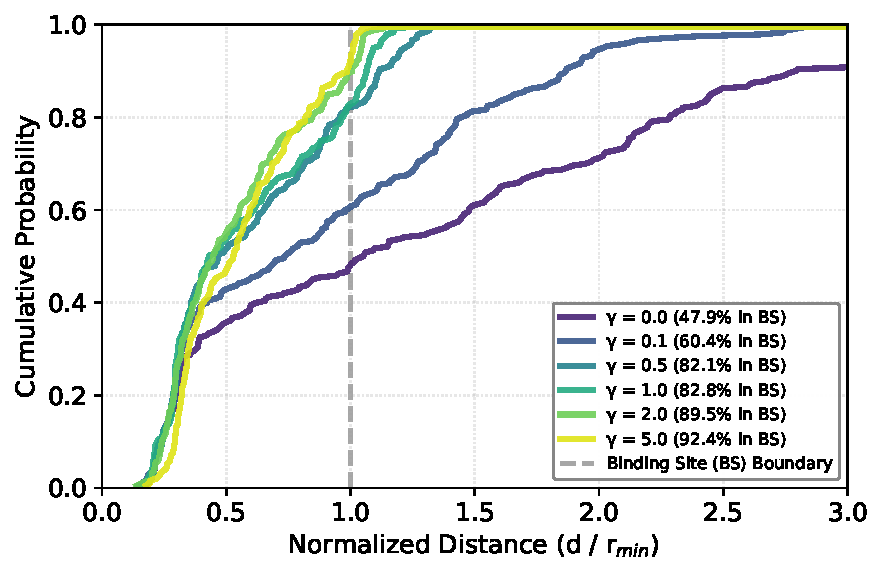
\includegraphics[width=0.85\textwidth]{cdf_plot_with_boundary_info.pdf}
\caption{Effect of binding site conditioning strength ($\gamma$) on pose sampling distribution. Cumulative distribution functions show the fraction of poses within a given normalized distance ($d/r_\mathrm{min}$) from the binding site center, aggregated across five Posebusters targets (7KFO, 7M41, 7AKL, 7XEK, 7NF3; 40 poses per target per $\gamma$ value; 1,200 total poses). The vertical dashed line indicates the binding site boundary. Percentages in the legend report the fraction of poses within this boundary. Increasing $\gamma$ progressively shifts probability mass toward the binding site, with $\gamma = 1$ (default) achieving 82.8\% occupancy while maintaining sampling diversity.}
\label{fig:gamma_cdf}
\end{figure}

\clearpage
\section{Table S1: AF2-DUD-E enrichment results for all methods}

\small
\begin{longtable}{@{\extracolsep{\fill}}lcccccc@{}}
\toprule
Target & \multicolumn{2}{c}{DiffDock-Glide ($\gamma=1$)} & \multicolumn{2}{c}{DiffDock-Confidence ($\gamma=1$)} & \multicolumn{2}{c}{Glide Confgen} \\
\cmidrule(lr){2-3} \cmidrule(lr){4-5} \cmidrule(lr){6-7}
 & EF 1\% & BEDROC & EF 1\% & BEDROC & EF 1\% & BEDROC \\
\midrule
\endfirsthead
\multicolumn{7}{c}%
{{\bfseries Table \thetable\ continued from previous page}} \\
\toprule
Target & \multicolumn{2}{c}{DiffDock-Glide ($\gamma=1$)} & \multicolumn{2}{c}{DiffDock-Confidence ($\gamma=1$)} & \multicolumn{2}{c}{Glide Confgen} \\
\cmidrule(lr){2-3} \cmidrule(lr){4-5} \cmidrule(lr){6-7}
 & EF 1\% & BEDROC & EF 1\% & BEDROC & EF 1\% & BEDROC \\
\midrule
\endhead
\midrule \multicolumn{7}{r}{{Continued on next page}} \\ \midrule
\endfoot
\bottomrule
\endlastfoot
aces & 3.8 & 0.091 & 2.0 & 0.030 & 6.6 & 0.121 \\
akt2 & 30.0 & 0.607 & 9.4 & 0.192 & 24.0 & 0.426 \\
ampc & 0.0 & 0.009 & 4.1 & 0.033 & 6.1 & 0.075 \\
bace1 & 37.0 & 0.633 & 13.0 & 0.199 & 25.0 & 0.446 \\
braf & 18.0 & 0.316 & 17.0 & 0.275 & 13.0 & 0.203 \\
cdk2 & 11.0 & 0.232 & 8.2 & 0.149 & 5.3 & 0.091 \\
dpp4 & 3.9 & 0.057 & 0.0 & 0.004 & 4.5 & 0.058 \\
egfr & 16.0 & 0.271 & 4.0 & 0.071 & 11.0 & 0.185 \\
fa10 & 22.0 & 0.608 & 16.0 & 0.406 & 15.0 & 0.427 \\
fabp4 & 44.5 & 0.512 & 8.5 & 0.149 & 5.5 & 0.200 \\
gria2 & 8.9 & 0.163 & 6.3 & 0.097 & 7.0 & 0.111 \\
hs90a & 5.7 & 0.091 & 14.0 & 0.253 & 6.9 & 0.102 \\
igf1r & 20.0 & 0.400 & 6.8 & 0.120 & 2.7 & 0.047 \\
ital & 0.73 & 0.016 & 0.0 & 0.001 & 3.6 & 0.059 \\
mapk2 & 14.0 & 0.242 & 35.0 & 0.599 & 30.0 & 0.491 \\
met & 7.8 & 0.125 & 4.8 & 0.070 & 11.0 & 0.180 \\
mk10 & 18.0 & 0.340 & 5.8 & 0.130 & 16.0 & 0.274 \\
mk14 & 18.0 & 0.323 & 8.8 & 0.149 & 11.0 & 0.195 \\
ppard & 22.0 & 0.437 & 0.83 & 0.021 & 10.0 & 0.214 \\
pparg & 1.2 & 0.019 & 1.7 & 0.027 & 2.9 & 0.010 \\
ptn1 & 25.0 & 0.530 & 4.6 & 0.097 & 23.0 & 0.427 \\
rxra & 42.0 & 0.732 & 29.0 & 0.530 & 51.0 & 0.836 \\
tgfr1 & 19.0 & 0.325 & 27.0 & 0.421 & 6.8 & 0.118 \\
thrb & 0.0 & 0.000 & 0.0 & 0.000 & 4.6 & 0.007 \\
try1 & 35.0 & 0.618 & 5.6 & 0.109 & 18.0 & 0.361 \\
tryb1 & 13.0 & 0.288 & 1.3 & 0.016 & 12.0 & 0.270 \\
vgfr2 & 14.0 & 0.275 & 9.5 & 0.193 & 6.6 & 0.129 \\
\midrule
\textbf{Average} & \textbf{16.7} & \textbf{0.306} & \textbf{9.0} & \textbf{0.161} & \textbf{12.6} & \textbf{0.225} \\
\end{longtable}

\bibliographystyle{plain}
\bibliography{main}

\end{document}
